\section{Empacotamento}
Nesta seção, a 4 seção do artigo \cite{lw23I} é exposta resumidamente com comentários sobre a implementação.  

\paragraph{Definições} Seja $K = K_1 \otimes K_2 \otimes K_3$ um corpo tensorial de três corpos linearmente disjuntos, e $\mathcal{R}_1, \mathcal{R}_2, \mathcal{R}_3$ sejam seus anéis de inteiros, respectivamente. Conclui-se que o anel de inteiros de $K$ (denotado como $\mathcal{R}$) é isomorfo a $\mathcal{R}_1 \otimes \mathcal{R}_2 \otimes \mathcal{R}_3$. Além disso, 

\begin{itemize}
    \item $K_{12}$ e $K_{13}$ denotam $K_1 \otimes K_2$ e $K_1 \otimes K_3$, respectivamente.
    \item $\mathcal{R}$, $\mathcal{R}_{12}$ e $\mathcal{R}_{13}$ denotam os anéis de inteiros de $K$, $K_{12}$, e $K_{13}$, respectivamente. Sabe-se que $\mathcal{R} \equiv \mathcal{R}_1 \otimes \mathcal{R}_2 \otimes \mathcal{R}_3$, $\mathcal{R}_{12} \equiv \mathcal{R}_1 \otimes \mathcal{R}_2$, e $\mathcal{R}_{13} \equiv \mathcal{R}_1 \otimes \mathcal{R}_3$.
    \item Sejam $(v_1, v_2, \ldots, v_\rho)$ e $(w_1, w_2, \ldots, w_\tau)$ algumas $\mathbb{Z}$-bases de $\mathcal{R}_2$ e $\mathcal{R}_3$, respectivamente, onde $\rho$ e $\tau$ são os graus dos anéis $\mathcal{R}_2$ e $\mathcal{R}_3$.
    \item Denotamos $(v_1^\vee, v_2^\vee, \ldots, v_\rho^\vee)$ e $(w_1^\vee, w_2^\vee, \ldots, w_\tau^\vee)$ como as correspondentes $\mathbb{Z}$-bases dos espaços duais $\mathcal{R}_2^\vee$ e $\mathcal{R}_3^\vee$, respectivamente.
    \item Seja $r = \min(\rho, \tau)$, o número máximo de slots que nosso método pode empacotar.
    \item Denotamos as funções de traço (com respeito a diferentes subcorpos subjacentes) como
    \[ \mathrm{Tr}_{K/K_{12}}: K \rightarrow K_{12} \text{ e } \mathrm{Tr}_{K/K_{13}}: K \rightarrow K_{13} \]
\end{itemize}

\subsection{Empacotamento de \textit{plaintext}}
 O algoritmo recebe $r$ mensagens $(x_1, \ldots, x_r) \in \mathcal{R}_1$ e um índice para um dos quatro modos: (1) $\mathcal{R}_{12}$, (2) $\mathcal{R}_{13}$, 
 (3) $\mathcal{R}_{12} \rightarrow \mathcal{R}_{13}$, e (4) $\mathcal{R}_{13} \rightarrow \mathcal{R}_{12}$, ,modos esses mantidos exatamente
 na implementação. O resultado da função é: 

 \begin{itemize}
    \item Modo 1: saída $\sum_{i=1}^r x_i \cdot v_i \in \mathcal{R}_{12}$.
    \item Modo 2: saída $\sum_{i=1}^r x_i \cdot w_i \in \mathcal{R}_{13}$.
    \item Modo 3: saída $\sum_{i=1}^r x_i \cdot v_i^\vee w_i \in \mathcal{R}_1 \otimes \mathcal{R}_2^\vee \otimes \mathcal{R}_3$.
    \item Modo 4: saída $\sum_{i=1}^r x_i \cdot w_i^\vee v_i \in \mathcal{R}_1 \otimes \mathcal{R}_2 \otimes \mathcal{R}_3^\vee$.
\end{itemize}
O algoritmo de empacotamento anexa um índice ao seu modo.

-- \textbf{Adição.} O algoritmo recebe duas codificações, nomeadamente $(x, \text{modo}_1)$, $(y, \text{modo}_2)$, e produz $(x+y, \text{modo}_1)$ se $\text{modo}_1 = \text{modo}_2$, caso contrário $\perp$.

-- \textbf{Multiplicação.} O algoritmo recebe duas codificações, nomeadamente $(x, \text{modo}_1)$ e $(y, \text{modo}_2)$, e faz uma das seguintes operações, selecionada pelos modos.
\begin{itemize}
    \item $\text{modo}_1 = 1 \text{ e } \text{modo}_2 = 3$: saída $\mathrm{Tr}_{K/K_{13}}(xy) \in \mathcal{R}_{13}$.
    \item $\text{modo}_1 =3 \text{ e } \text{modo}_2 = 1$: saída $\mathrm{Tr}_{K/K_{12}}(xy) \in \mathcal{R}_{12}$.
    \item $\text{modo}_1 = 2 \text{ e } \text{modo}_2 = 4$: saída $\mathrm{Tr}_{K/K_{13}}(xy) \in \mathcal{R}_{13}$.
    \item $\text{modo}_1 = 4\text{ e } \text{modo}_2 = 2$: saída $\mathrm{Tr}_{K/K_{12}}(xy) \in \mathcal{R}_{12}$.
    \item Caso contrário $\perp$.
\end{itemize}

Essas operações estão implementadas no github no directório plaintext\_operations. 

\paragraph{Nota:} Para o plaintexts e ciphertexts, seus elementos vão ser armazenados em $\mcR$ ao invés do dual. Por exemplo, para o criptograma 
$a \in \mathcal{R}_1 \otimes \mathcal{R}_2^\vee \otimes \mathcal{R}_3$, vamos armazenar o criptograma $aP \in \mcR$ onde $P = \rho$. Esta multiplicação
garante que o elemento tem representação única em $\mcR$ e facilita a implementação.
\subsection{Empacotamento de \textit{ciphertexts}}

Para esta seção utilizamos uma função chamada de Eval-Trace, que recebe um criptograma cifrado em RLWE ou RGSW e devolve outro cifrando o traço da mensagem, ou seja:
$$
\text{Eval-Tr}_{K/K_{13}} : \text{RLWE}_s(\mu) \rightarrow \text{RLWE}_s(\text{Tr}_{K/K_{13}}(\mu))
$$

Tome-a como \textit{black-box} na próxima seção o seu funcionamento vai ser detalhado, então vamos descrever os empacotamentos.


RGSW-Pack. O algoritmo recebe como entrada $r$ RGSW ciphertexts $C_1, C_2, \ldots, C_r \in \mathcal{R}^{2 \times 2^{2\ell}}$, onde cada $C_i$ é RGSW$(\mu_i)$, para $\mu_i \in \mathcal{R}_1$ - no caso da implementação,
recebe o elemento correspondente em $\mcR$, $\mu_i' = \mu_i \otimes 1$ mas seu funcionamento teórico permanece - e um índice para um dos quatro modos: (1) $\mathcal{R}_{12}$, (2) $\mathcal{R}_{13}$, (3) $\mathcal{R}_{12} \rightarrow \mathcal{R}_{13}$ e (4) $\mathcal{R}_{13} \rightarrow \mathcal{R}_{12}$. O algoritmo produz um RGSW ciphertext empacotado,
de modo descrito a seguir
\begin{itemize}
    \item Modo 1: saída $\sum_{i=1}^r C_i \cdot v_i \in \mathcal{R}^{2 \times 2^\ell}$.
    \item Modo 2: saída $\sum_{i=1}^r C_i \cdot w_i \in \mathcal{R}^{2 \times 2^\ell}$.
    \item Modo 3: saída $\sum_{i=1}^r C_i \cdot v_i^\vee w_i \in (\mathcal{R}_1 \otimes \mathcal{R}_2^\vee \otimes \mathcal{R}_3)^{2 \times 2^\ell}$.
    \item Modo 4: saída $\sum_{i=1}^r C_i \cdot w_i^\vee v_i \in (\mathcal{R}_1 \otimes \mathcal{R}_2 \otimes \mathcal{R}_3^\vee)^{2 \times 2^\ell}$.
\end{itemize}
O algoritmo de empacotamento anexa um índice ao seu modo na clara.

-- RLWE-Pack. O algoritmo recebe $r$ RLWE ciphertexts $e_1, e_2, \ldots, e_r$, onde cada $e_i \in \text{RLWE}(\mu_i)$, para $\mu_i \in \mathcal{R}_1$ e um índice para um dos quatro modos iguais aos de RGSW-packing. O algoritmo produz uma codificação dos RLWE ciphertexts.

\begin{itemize}
    \item Modo 1: saída $\sum_{i=1}^r c_i \cdot v_i \in \mathcal{R}_{12}$.
    \item Modo 2: saída $\sum_{i=1}^r c_i \cdot w_i \in \mathcal{R}_{13}$.
    \item Modo 3: saída $\sum_{i=1}^r c_i \cdot v_i^\vee w_i \in (\mathcal{R}_1 \otimes \mathcal{R}_2^\vee \otimes \mathcal{R}_3)$.
    \item Modo 4: saída $\sum_{i=1}^r c_i \cdot w_i^\vee v_i \in (\mathcal{R}_1 \otimes \mathcal{R}_2 \otimes \mathcal{R}_3^\vee)$.
\end{itemize}
O modo é incluído no criptograma às claras e os elementos no dual são passados para o anel principal $\mcR$ como descrito na sessão anterior.

-- Adição para RGSW-encodings: O algoritmo recebe duas codificações RGSW, nomeadamente $(C_1, \text{modo}_1)$, $(C_2, \text{modo}_2)$, e produz $(C_1 + C_2, \text{modo}_1)$ se $\text{modo}_1 = \text{modo}_2$, caso contrário $\perp$.

-- Adição para RLWE-encodings: O algoritmo recebe duas codificações RLWE, nomeadamente $(e_1, \text{modo}_1)$, $(e_2, \text{modo}_2)$, e produz $(e_1 + e_2, \text{modo}_1)$ se $\text{modo}_1 = \text{modo}_2$, caso contrário $\perp$.

-- Produto Homomórfico para RGSW-RGSW: O algoritmo recebe dois criptogramas RGSW empacotados, nomeadamente $(C_1, \text{modo}_1)$ e $(C_2, \text{modo}_2)$, e então calcula $C = C_1 \cdot G^{-1}(C_2)$. Então ele retorna:

\begin{itemize}
    \item $\text{modo}_1 = 1 \text{ e } \text{modo}_2 = 3$: saída $\text{Eval-Tr}_{K/K_{13}}(C)$.
    \item $\text{modo}_1 = 2 \text{ e } \text{modo}_2 = 4$: saída $\text{Eval-Tr}_{K/K_{12}}(C)$.
    \item $\text{modo}_1 = 3 \text{ e } \text{modo}_2 = 1$: saída $\text{Eval-Tr}_{K/K_{13}}(C)$.
    \item $\text{modo}_1 = 4 \text{ e } \text{modo}_2 = 2$: saída $\text{Eval-Tr}_{K/K_{12}}(C)$.
    \item Caso contrário $\perp$.
\end{itemize}
-- Eval-Mult (Produto Externo para RGSW-RLWE). O algoritmo recebe uma codificação RGSW $(C_1, \text{modo}_1)$ e uma codificação RLWE $(e_2, \text{modo}_2)$, e então calcula $C = C_1 \cdot g^{-1}(c_2)$. Então, retorna para cada caso:
\begin{itemize}
    \item $\text{modo}_1 = 1 \text{ e } \text{modo}_2 = 3$: saída $\text{Eval-Tr}_{K/K_{13}}(C)$.
    \item $\text{modo}_1 = 2 \text{ e } \text{modo}_2 = 4$: saída $\text{Eval-Tr}_{K/K_{12}}(C)$.
    \item $\text{modo}_1 = 3 \text{ e } \text{modo}_2 = 1$: saída $\text{Eval-Tr}_{K/K_{13}}(C)$.
    \item $\text{modo}_1 = 4 \text{ e } \text{modo}_2 = 2$: saída $\text{Eval-Tr}_{K/K_{12}}(C)$.
    \item Caso contrário $\perp$.
\end{itemize}


\paragraph{Por que não empacotar as mensagens em um criptograma?}

O ruído acaba crescendo exponencialmente ao realizar múltiplos produtos externos consecutivamente. Para mais detalhes, 
vamos utilizar resultados das seções seguintes. Se decidirmos empacotar mensagens a expressão de um produto externo será:
$$
Tr_{K/K_{13}} (e_1g^{-1}(c_2) + \mu_1 e_2) + e'
$$
onde $e_1, e_2$ são os ruídos do criptograma RGSW e RLWE respectivamente. Como o ruído não possui nenhuma propriedade especial 
em relação as bases $v_i, w_i$ é válido afirmar que a sua norma vai crescer proporcional a um fator $\phi(p_2^{n_2})$. Portanto, após 
$k$ aplicações de produto externo, a norma final será limitada com um fator de $\approx \phi(p_2^{n_2})^{k/2} \phi(p_3^{n_3})^{k/2}$
que é exponencial. Tal crescimento pode ser verificado via o gráfico a seguir:

\begin{figure}[htbp]
    \centering
    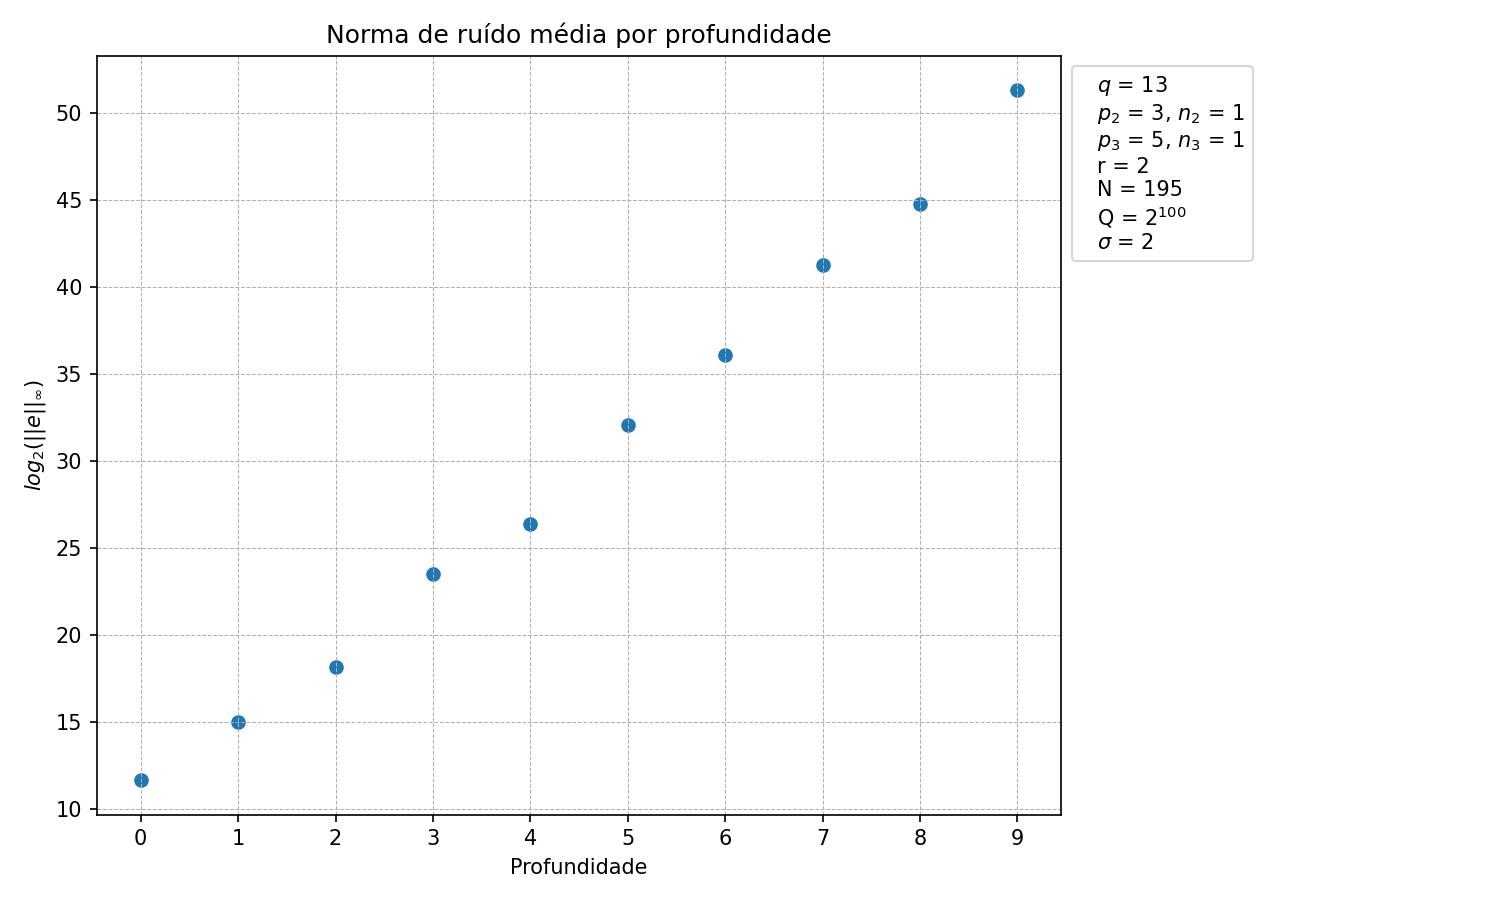
\includegraphics[width=0.8\textwidth]{images/wrong_packing.jpg}
    \caption{Crescimento do ruído pela quantidade de produtos externos com empacotamento errado.}
    \label{fig:wrong_packing}
\end{figure}